\documentclass[conference]{IEEEtran}
\IEEEoverridecommandlockouts

\usepackage{cite}
\usepackage{amsmath,amssymb,amsfonts}
\usepackage{graphicx}
\usepackage{textcomp}
\usepackage{xcolor}
\usepackage{url}
\usepackage{enumitem}
\usepackage{booktabs}

\begin{document}

\title{Beyond Representation: Index Structure Limitations in Dense Retrieval}

\author{\IEEEauthorblockN{Alessandro Magnani}
\IEEEauthorblockA{\textit{Independent Researcher}\\
ale.magnani@gmail.com}
}

\maketitle

\begin{abstract}
Dense retrieval relies on approximate nearest-neighbor (ANN) indices such as HNSW and IVF for practical deployment. Prior theoretical work has focused on the \emph{representational} capacity of dense embeddings; we show that the \emph{indexing} stage imposes a separate, quantifiable bottleneck. We introduce \emph{indexing bias}---the systematic gap between exact and approximate retrieval probability---and derive a centroid-dilution bound linking IDF-weighted token rarity, embedding dimensionality, and cluster granularity. We then isolate index-induced failures empirically by holding the representation fixed (random-projection trigram embeddings at varying dimensions) and varying only the indexing structure on Home Depot product search and MS MARCO Passage. On so-called \emph{spear-fishing} queries---those depending on identifiers or rare terms---switching from exact to HNSW search forfeits up to $63\%$ of the achievable Recall@10, versus less than $2\%$ for standard semantic queries. Increasing embedding dimensionality reduces representation noise but does not close this index-induced gap. The results reframe the sparse-vs-dense trade-off as a joint choice of representation and indexing, with direct implications for production retrieval stacks where part-number, SKU, and named-entity queries are operationally important.
\end{abstract}

\begin{IEEEkeywords}
dense retrieval, approximate nearest neighbor search, index structures, information retrieval, service quality
\end{IEEEkeywords}

\section{Introduction}
Information retrieval (IR) has seen a paradigm shift with the advent of neural dense retrieval methods that use learned embeddings \cite{ma2022survey}, challenging traditional sparse retrieval methods based on lexical term matching \cite{karpukhin2020dense, xiong2021approximate}. As IR systems increasingly serve as critical components in various service ecosystems—from e-commerce platforms and enterprise search to digital assistants and knowledge management services—their reliability and performance across diverse query patterns directly impacts user satisfaction and service quality.

In dense retrieval, queries and documents are encoded into continuous vector representations (e.g., via BERT-based encoders) and relevant items are found by nearest-neighbor search in embedding space. This approach has revolutionized many information services by improving semantic understanding and results relevance. In contrast, sparse retrieval represents text as high-dimensional sparse vectors (often TF-IDF or BM25 term weights) and relies on inverted indexes to match overlapping terms, with recent advances also incorporating learned sparse representations \cite{formal2021splade}.

Theoretical analyses, notably the work by Tay et al.\ \cite{tay2020sparse} using random projection techniques, suggest that dense representations, given sufficient dimensionality, possess the theoretical capacity to approximate or even surpass traditional sparse methods. However, the practical scalability of dense retrieval in service environments hinges critically on Approximate Nearest Neighbor (ANN) search algorithms (e.g., HNSW, IVF). While much research has focused on the representational power of embeddings, the fundamental limitations imposed by these necessary ANN index structures themselves remain relatively underexplored. This gap becomes particularly concerning for service engineers designing systems that must handle heterogeneous query patterns from diverse user populations.

This paper argues that ANN index structures introduce significant bottlenecks, particularly for what we term ``spear fishing'' queries—those whose relevance depends critically on rare terms or specific, non-semantic patterns (like identifiers). These queries often correspond to documents lying in sparser regions of the embedding space but may represent important user service interactions such as precise product searches or specific information lookup tasks. We extend prior theoretical work \cite{tay2020sparse, fan2022information} by analyzing how the approximations inherent in common ANN indices systematically disadvantage such queries.

We make the following contributions:
\begin{itemize}
    \item We formalize the concept of ``spear fishing'' queries and demonstrate theoretically why standard ANN indices (IVF and HNSW) struggle with them, \emph{independent of the representation's theoretical capacity}.

    \item We derive a \emph{centroid-dilution bound} that links IDF-weighted token rarity, embedding dimensionality $d$, and clustering granularity to the probability that an IVF centroid fails to carry a rare token's signal above the Johnson--Lindenstrauss noise floor.

    \item We isolate index-induced failure empirically by comparing exact (Flat) and approximate (IVF, HNSW) search on a controlled three-axis design (two datasets $\times$ three query types $\times$ three embedding dimensions), and quantify the resulting \emph{indexing bias}.

    \item We show that the gap is disproportionately large for ID and rare-term queries and that, unlike representation-level limitations, this gap does not vanish at higher embedding dimensionality.
\end{itemize}

\noindent\textit{What is new versus prior work.} Tay et al.~\cite{tay2020sparse} and Fan et al.~\cite{fan2022information} analyze \emph{representation-level} capacity of dense vectors. We complement this with an \emph{index-level} analysis: we hold the representation fixed (via random-projection trigram embeddings of varying dimension) and vary only the indexing structure, so that every observed degradation can be attributed to the index. Sec.~\ref{sec:theory} formalizes this separation; Sec.~\ref{sec:experiments} tests it.

\section{Background and Related Work}

\subsection{Dense Retrieval Approaches}
Dense retrieval models map queries and documents to continuous vector representations, typically using neural networks. Notable approaches include the Dense Passage Retriever (DPR) \cite{karpukhin2020dense}, which uses separate BERT encoders for queries and documents, ANCE \cite{xiong2021approximate}, which employs hard negative mining to improve representation learning, and Sentence-BERT \cite{reimers2019sentencebert}, which adapts BERT for efficient semantic similarity comparison. These models are trained on large datasets with relevance labels, learning to place semantically related queries and documents close in embedding space.

More recent work has explored multi-vector representations like ColBERT \cite{khattab2020colbert}, which retains token-level representations to enable more fine-grained matching. While effective, these approaches generally require significant training data and computational resources.

\subsection{Theoretical Capabilities of Dense Representations}
Tay et al.\ \cite{tay2020sparse} demonstrated that dense representations can theoretically approximate sparse retrieval performance using random projections. Their analysis showed that with sufficient dimensionality, dense vectors can capture the same information as sparse vectors. They introduced a latent-based dual encoder model that combines these theoretical insights with modern neural architectures, and proposed multi-vector representations to address some limitations of single-vector approaches.

Fan et al.\ \cite{fan2022information} conducted an information-theoretic analysis of dense representations to measure how much variability in queries is preserved, finding that dense models have lower capacity for tail information than sparse ones. This theoretical limitation helps explain empirical observations about dense retrievers struggling with rare entities or terms.

\subsection{Index Structures for Dense Retrieval}
To make dense retrieval practical at scale, approximate nearest neighbor (ANN) indexing is essential \cite{johnson2019billion}. Two families dominate in practice and frame our analysis: \emph{Hierarchical Navigable Small World} (HNSW) graphs~\cite{malkov2019efficient}, which build a multi-layer proximity graph and search it greedily, and \emph{Inverted File} (IVF) indices, optionally combined with Product Quantization \cite{jegou2010product}, which cluster documents by k-means and probe only the closest centroids at query time. Both achieve speed via approximations that work well on average but can systematically fail on tail cases. Lin \cite{lin2024dense} notes that HNSW degrades retrieval quality by a small (often-unreported) amount relative to exact search; we argue this small \emph{average} loss masks a much larger loss concentrated on a specific query population.

\subsection{Research Gap}
Benchmarks such as BEIR \cite{thakur2021beir} document dense-retrieval failures on out-of-distribution and entity-heavy queries, and fairness work \cite{zhan2021understanding} hints that index-level effects are involved, but the contribution of the ANN index itself is rarely isolated. The interaction between representation quality and index approximation quality remains open: even with embeddings of sufficient capacity, ANN search may introduce unavoidable per-query failure modes. This paper isolates the index contribution by construction.

\section{Theoretical Analysis}\label{sec:theory}

We extend the random-projection view of dense retrieval \cite{tay2020sparse} to the indexing stage. The argument has three steps: (i)~a representation has a token-level signal whose magnitude depends on IDF weight and dimensionality; (ii)~exact search preserves this signal up to JL distortion; (iii)~practical ANN structures introduce a \emph{second}, qualitatively different distortion that disproportionately attenuates rare-token signals. Our contributions in this section are the centroid-dilution bound (Eq.~\eqref{eq:centroid_signal_mag}), the indexing-bias decomposition (Eq.~\eqref{eq:indexing_bias}), and the four testable predictions in Sec.~\ref{sec:predictions} that the experiments target directly.

\subsection{Foundational Concepts}

We begin by outlining the core components of our model:

\begin{enumerate}[label=(\arabic*)]
\item \textbf{Document Representation:} Following Tay et al.\ \cite{tay2020sparse}, each document $d$ is represented in an IDF-based manner as a sum of its token embeddings:
\begin{equation}
f(d) = \sum_{t\in d} \alpha_t\, \phi(t)
\label{eq:doc_rep}
\end{equation}
where $\phi(t)$ is the dense embedding for token $t$ (assumed unit-norm, $\|\phi(t)\| = 1$), and $\alpha_t$ is its IDF weight.

\item \textbf{Rare Token Characteristics:} Consider a rare token $t^*$ appearing infrequently in the corpus. Let $M$ be the total number of documents and $n_{t^*}$ be the number of documents containing $t^*$. A common IDF weight is:
\begin{equation}
\alpha_{t^*} = \log\left(\frac{M}{n_{t^*}}\right)
\label{eq:idf_weight}
\end{equation}
For rare tokens ($n_{t^*} \ll M$), this weight $\alpha_{t^*}$ is large, meaning the token carries significant identifying information in sparse models like BM25.

\item \textbf{Dimensionality Reduction via Random Projection:} High-dimensional embeddings (dimension $V$) are often projected to lower dimension $d$ using random projection matrix $W\in \mathbb{R}^{d\times V}$. The Johnson-Lindenstrauss lemma \cite{johnson1984extensions} guarantees distance preservation: for any vector $x$,
\begin{equation}
(1-\epsilon)\|x\|^2 \leq \|W x\|^2 \leq (1+\epsilon)\|x\|^2
\label{eq:jl_lemma}
\end{equation}
with high probability. The distortion $\epsilon$ is bounded by:
\begin{equation}
\epsilon \approx \sqrt{\frac{\log V}{d}}
\label{eq:jl_error_bound}
\end{equation}
\end{enumerate}

\subsection{Signal Loss for Rare Tokens}

In dense retrieval, the relevance signal for token $t^*$ within document embedding $f(d)$ is carried by term $\alpha_{t^*} \phi(t^*)$. When documents are grouped by indexing structures (e.g., clusters), the effective signal strength of $t^*$ becomes crucial.

Consider an aggregate representation $c$ (e.g., cluster centroid) from document set $C$. The expected contribution of rare token $t^*$ to aggregate $c$ depends on its IDF weight $\alpha_{t^*}$ and prevalence $p$ within group $C$. Let $p$ be the fraction of documents in $C$ containing $t^*$. The signal magnitude $\Delta_{t^*}$ is proportional to $\alpha_{t^*}^2 p$.

The signal becomes lost when its magnitude is overwhelmed by projection noise:
\begin{equation}
\|\Delta_{t^*}\| \lesssim \epsilon \approx \sqrt{\frac{\log V}{d}}
\label{eq:signal_loss_general}
\end{equation}

This highlights a fundamental tension: rare but important tokens (high $\alpha_{t^*}$) might be lost if sparsely distributed within index groups (low $p$) or if projection is too aggressive (high $\epsilon$).

\subsection{Indexing Bias}

Exact nearest neighbor search over dense vectors $z = Wf(d)$ would preserve the relevance signal, subject only to JL distortion $\epsilon$. However, exact search is computationally infeasible for large corpora. Practical dense retrieval relies on ANN algorithms.

ANN algorithms achieve speed through approximations, leading to \textbf{indexing bias}: a systematic discrepancy between retrieval probability using exact versus approximate search:
\begin{equation}
\text{Bias}(q, d) = P_{\text{exact}}(\text{ret}(q, d)) - P_{\text{approx}}(\text{ret}(q, d))
\label{eq:indexing_bias}
\end{equation}

This bias arises because ANN methods often favor certain regions:
\begin{itemize}
    \item \textbf{Density Preference:} Many ANN methods navigate densely populated regions more effectively. Outliers or documents in sparse regions may be harder to find.
    
    \item \textbf{Approximation Errors:} Quantization, graph traversal heuristics, and limited probing introduce errors where true nearest neighbors might be missed.
\end{itemize}

Indexing bias particularly harms ``spear fishing'' queries, where relevance hinges on specific, potentially rare information defining less populated regions in embedding space.

\subsection{Index-Specific Bottlenecks}

\subsubsection{IVF / Clustering-based Indices}

Inverted File (IVF) indices partition the document embedding space into $N$ clusters. Each cluster $C$ is represented by centroid $c$:
\begin{equation}
c = \frac{1}{|C|}\sum_{d\in C} f(d)
\label{eq:centroid_calc}
\end{equation}

During search for query $q$, only a subset $G = n_{\text{probes}}$ of clusters with closest centroids are searched.

This suffers from two issues for rare tokens $t^*$:

\textbf{1. Centroid Dilution:} The contribution $\Delta_{t^*}$ of rare token $t^*$ to centroid $c$ is averaged over all $|C| \approx M/N$ documents. Assuming $t^*$ appears in $n_{t^*,C}$ documents within cluster $C$, probability $p = n_{t^*,C} / |C|$. The magnitude is:
\begin{equation}
\|\Delta_{t^*}\| \approx \alpha_{t^*}^2 p = \left[\log\left(\frac{M}{n_{t^*}}\right)\right]^2 \cdot \frac{n_{t^*,C}}{M/N}
\label{eq:centroid_signal_mag}
\end{equation}

Even in the best case where all occurrences fall into one cluster, if this magnitude falls below noise threshold $\epsilon$, the centroid will not reflect $t^*$ presence.

\textbf{2. Cluster Selection Failure:} Retrieval requires selecting correct cluster(s). If the $t^*$ signal in the centroid is diluted, the correct cluster may not be among top $G$ probed. The probability is roughly:
\begin{equation}
\mathbb{P}(\text{correct cluster}) \approx \frac{G}{N} = \frac{n_{\text{probes}}}{n_{\text{lists}}}
\label{eq:ivf_probe_prob}
\end{equation}

\subsubsection{HNSW / Graph-based Indices}

HNSW \cite{malkov2019efficient} builds multi-layer graphs where nodes are document embeddings. Search traverses the graph greedily towards the query embedding.

HNSW faces challenges with rare-token queries due to:

\textbf{1. Sparse Connectivity:} Embeddings dominated by rare tokens might reside in sparsely populated ``outlier'' regions with poor graph connectivity. Search might fail to navigate into these regions.

\textbf{2. Traversal Errors:} Greedy search is heuristic. Even with good connectivity, the search path might diverge, especially when subtle differences distinguish the target.

The retrieval probability depends on both similarity and graph structure:
\begin{equation}
P_{\text{approx}}(\text{ret}(q, d)) = g(\text{sim}(z_q, z_d), \text{conn}(z_d))
\label{eq:hnsw_retrieval_prob}
\end{equation}

For rare queries, $z_d$ might be in low-density/poorly-connected regions, reducing $P_{\text{approx}}$ significantly.

\begin{table}[t]
\centering
\small
\caption{Comparative Analysis of Index Limitations}
\label{tab:comparison_revised}
\begin{tabular}{lccc}
\toprule
\textbf{Index} & \textbf{Efficiency} & \textbf{Common} & \textbf{Rare (Failure)} \\
\midrule
HNSW & High & Strong & Weak (Connectivity) \\
IVF & Moderate & Good & Weak (Dilution) \\
\bottomrule
\end{tabular}
\end{table}

\subsection{Testable Predictions}\label{sec:predictions}

This framework leads to four experimentally testable predictions, each tied to a specific experiment in Sec.~\ref{sec:experiments}:

\begin{enumerate}
\item \textbf{IVF Recall Scaling:} For rare-term and ID queries, IVF Recall@k should increase approximately linearly with probe ratio ($n_{\text{probes}}/n_{\text{lists}}$), but plateau below exact search due to centroid dilution.

\item \textbf{Exact vs.\ Approximate Gap:} The performance gap between exact and approximate search will be substantially larger for rare-term and ID queries than for standard semantic queries.

\item \textbf{Dimensionality Benefit:} Increasing embedding dimensionality $d$ should disproportionately benefit rare-term queries under ANN search by reducing projection noise $\epsilon$.

\item \textbf{Index Mechanism Differences:} Both IVF and HNSW underperform Flat search on rare queries, but failure patterns might differ, reflecting distinct mechanisms.
\end{enumerate}

\section{Experiments}\label{sec:experiments}

Our experimental design isolates index-induced failures by holding the representation family fixed and varying only the indexing structure. Concretely, we use unsupervised character-trigram embeddings projected to a controlled dimension; this lets us interpret any Flat$\to$ANN gap as an index effect rather than a representation effect.

\subsection{Setup}\label{sec:setup}

\paragraph{Datasets and corpus construction.}
We evaluate on two datasets chosen for contrasting query distributions:
\begin{itemize}
\item \textbf{Home Depot} (HD): from the public Home Depot product-search relevance corpus. We deduplicate by \texttt{product\_uid}, yielding $54{,}667$ unique product titles, and use the $11{,}795$ unique customer \texttt{search\_term} values with the provided product$\to$query relevance as ground truth.
\item \textbf{MS MARCO Passage v1.1} (MM): we use the \texttt{validation} split (10{,}047 queries) and flatten each query's candidate passage list into $82{,}360$ passage documents, marking the passage with \texttt{is\_selected=1} as relevant.
\end{itemize}

\paragraph{Query subsets.}
For each dataset we construct three query subsets, each capped at $1{,}000$ queries (random sampling with seed $42$ where applicable):
\begin{itemize}
\item \textbf{Standard}: real user queries with their provided relevance judgments.
\item \textbf{ID}: a random sample of document identifiers used as queries, with self-relevance ($q{=}d$). To enable retrieval on these IDs, the identifier string is prepended to each document's text when indexing this subset. This is the extreme ``spear fishing'' regime: relevance depends on a single low-frequency token.
\item \textbf{Rare}: generated queries consisting of unigrams or bigrams (alphabetic, length $>3$) that occur in at most $5$ documents of the corpus, with their containing documents as relevance set.
\end{itemize}

\paragraph{Embedding model.}
We use a fully unsupervised pipeline so no learned signal can confound the comparison: \texttt{HashingVectorizer} with $2^{18}{=}262{,}144$ buckets, character $3$-grams (\texttt{analyzer=`char'}, \emph{across-token} mode---we verified \texttt{`char\_wb'} gives qualitatively the same trends), followed by a sparse Johnson--Lindenstrauss projection (\texttt{SparseRandomProjection}, density $0.9$, seed $42$) to dimension $d\in\{256,512,1024\}$. Embeddings are L2-normalized so that L2 nearest-neighbor search is equivalent to cosine similarity.

\paragraph{Retrieval backends and parameter sweeps.} All dense methods use FAISS:
\begin{itemize}
\item \textbf{Flat}: exhaustive L2 search ($P_{\text{exact}}$ baseline).
\item \textbf{IVF}: \texttt{IndexIVFFlat} with $n_{\text{list}}\in\{200,500,1000\}$ k-means cells and $n_{\text{probe}}=\lceil n_{\text{list}}\cdot p\rceil$ for $p\in\{0.1,0.2,0.5\}$, giving nine $(n_{\text{list}},n_{\text{probe}})$ configurations per dimension.
\item \textbf{HNSW}: \texttt{IndexHNSWFlat} with $M{=}64$, \texttt{efConstruction}$\in\{100,200\}$, \texttt{efSearch}$=100$.
\item \textbf{BM25}: Anserini/Lucene via Pyserini~\cite{lin2021pyserini} with default parameters.
\end{itemize}

\paragraph{Metric and reproducibility.}
We report Recall@$10$ (we also compute Recall@$\{1,5,20,50,100\}$ with consistent trends). All numbers are aggregated over the $\le 1{,}000$ queries per subset. The full sweep (over $200$ runs per dataset across the cross-product of \{subset, dimension, index, sweep parameter\}) is deterministic given the seed; the released code generates all tables and figures from one JSON results file.

\subsection{IVF Degrades for Rare and ID Queries}

\begin{figure}[t]
\centerline{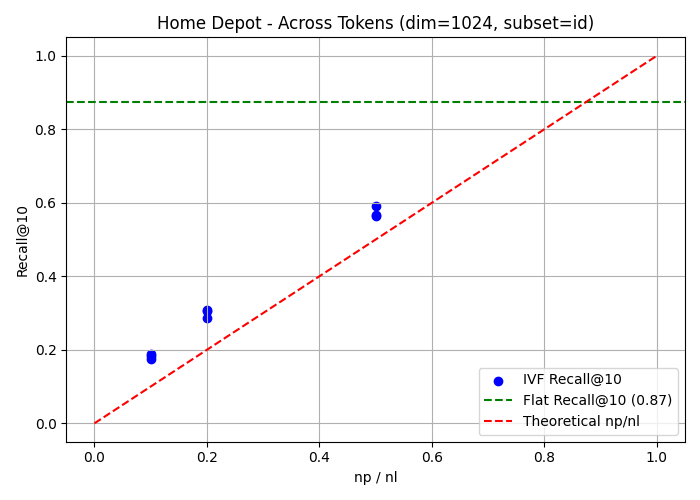
\includegraphics[width=\columnwidth]{figures/home_id_npnl.png}}
\centerline{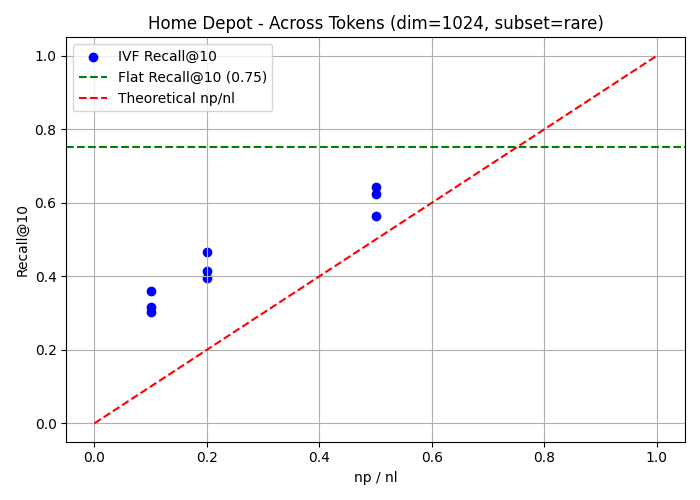
\includegraphics[width=\columnwidth]{figures/home_rare_npnl.png}}
\caption{Recall@10 vs.\ probe ratio (np/nl) for IVF and Flat on Home Depot (ID and Rare queries, dim=1024). Flat consistently outperforms IVF. IVF recall scales roughly linearly with probe ratio but remains significantly lower than Flat.}
\label{fig:npnl_recall}
\end{figure}

Figure~\ref{fig:npnl_recall} directly tests \textbf{Prediction 1} (IVF Recall Scaling) and provides evidence for \textbf{Prediction 2} (Exact vs.\ Approximate Gap).

As predicted, Recall@10 for IVF grows approximately linearly with probe ratio ($n_{\text{probes}}/n_{\text{lists}}$), reflecting increasing probability of searching the correct cluster. However, critically, even when probing a large fraction of clusters, IVF recall plateaus significantly below Flat search performance.

This persistent gap validates \textbf{Prediction 2} and points to index structure limitations. The linearity confirms cluster selection bottleneck, while the gap suggests that even when correct cluster is probed, retrieval often fails. This is attributed to \textbf{centroid dilution}, where the rare signal within the centroid is insufficient for robust retrieval.

\subsection{Trigram Embeddings on Standard Queries}

\begin{figure}[t]
\centerline{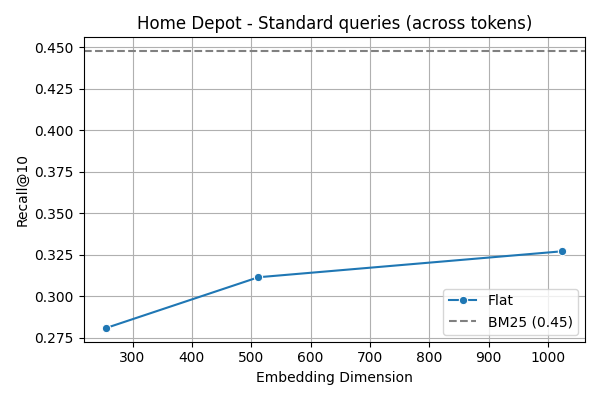
\includegraphics[width=\columnwidth]{figures/home_standard_dim.png}}
\centerline{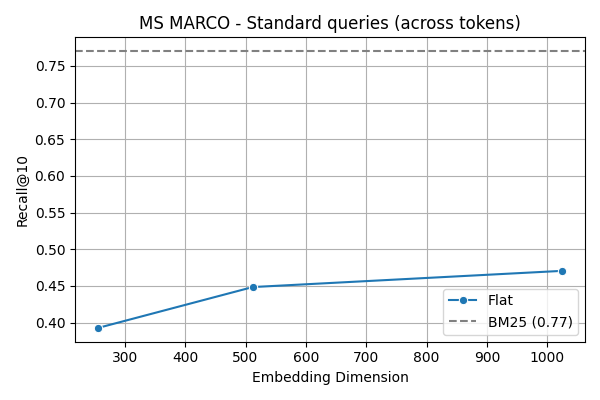
\includegraphics[width=\columnwidth]{figures/msmarco_standard_dim.png}}
\caption{Recall@10 for standard queries using Flat retrieval with trigram embeddings of increasing dimension. BM25 baseline shown as dashed line.}
\label{fig:standard_dim}
\end{figure}

Figure~\ref{fig:standard_dim} evaluates unsupervised trigram embeddings using exact (Flat) search on standard queries. On Home Depot, even 256-dim embeddings surpass BM25. On MS MARCO, performance improves with dimensionality, eventually outperforming BM25 at 1024 dimensions.

This confirms underlying dense representations have capacity for semantic retrieval. Performance increase with dimension aligns with expectation that lower JL distortion $\epsilon$ improves representation fidelity. However, effectiveness on standard queries with exact search contrasts sharply with failures for approximate search on rare/ID queries, emphasizing the bottleneck lies within the approximate index.

\subsection{Flat Search vs.\ Dimensionality}

\begin{figure}[t]
\centerline{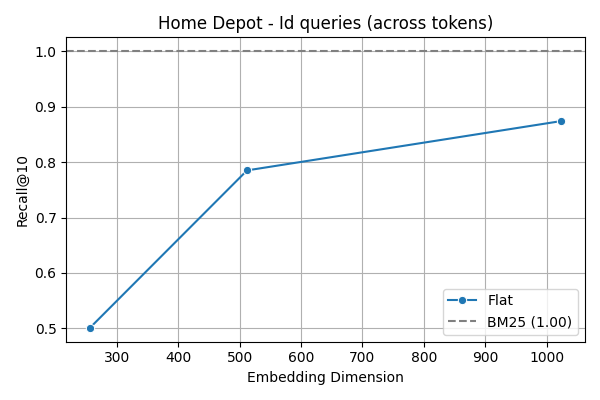
\includegraphics[width=\columnwidth]{figures/flat_dim_home_id.png}}
\centerline{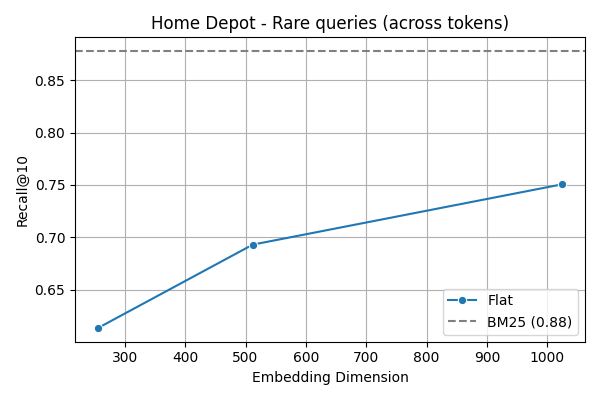
\includegraphics[width=\columnwidth]{figures/flat_dim_home_rare.png}}
\caption{Flat Recall@10 for ID and Rare queries (Home Depot) as function of embedding dimension. BM25 baseline shown.}
\label{fig:flat_dim_queries}
\end{figure}

Figure~\ref{fig:flat_dim_queries} examines dimensionality impact on exact (Flat) search for ID and Rare queries, testing \textbf{Prediction 3}.

Results show that even with exact search, increasing dimensionality generally improves or maintains high recall. For ID queries, performance is very high at 256 dimensions. For Rare queries, clearer benefit from increasing dimensions (256 to 512).

Theoretically, increasing $d$ reduces JL distortion $\epsilon$, improving rare token signal preservation. This confirms higher dimensionality makes underlying representation more robust for capturing rare signals, even before considering ANN approximations.

\subsection{Detailed Performance Comparison}

\begin{table}[t]
\centering
\small
\caption{Recall@10 for Best Configurations}
\label{tab:detailed-results}
\setlength{\tabcolsep}{4pt}
\begin{tabular}{llrrrr}
\toprule
\textbf{Dataset} & \textbf{Subset} & \textbf{Flat} & \textbf{IVF} & \textbf{HNSW} & \textbf{BM25} \\
\midrule
HD       & standard & 0.327 & 0.314 & 0.321 & 0.447 \\
HD       & id       & 0.874 & 0.590 & 0.327 & 1.000 \\
HD       & rare     & 0.751 & 0.642 & 0.619 & 0.878 \\
\midrule
MS MARCO & standard & 0.471 & 0.448 & 0.446 & 0.770 \\
MS MARCO & id       & 0.174 & 0.152 & 0.071 & 0.000$^{\dagger}$ \\
MS MARCO & rare     & 0.205 & 0.187 & 0.166 & 0.688 \\
\bottomrule
\end{tabular}
\\[2pt]
{\footnotesize Dense at $d{=}1024$, across-token trigrams, best ANN sweep.\\
$^{\dagger}$BM25 cannot tokenize compound passage IDs.}
\end{table}

Table~\ref{tab:detailed-results} validates \textbf{Predictions 2--4} at $d{=}1024$.

\textbf{Prediction 2 (Exact vs.\ Approximate gap).} The Flat$\to$HNSW gap is order-of-magnitude larger on spear-fishing subsets than on standard queries. On Home Depot, the gap is $0.006$ absolute (1.8\% relative) for standard queries, $0.132$ (17.5\% relative) for rare queries, and $0.547$ (62.6\% relative) for ID queries. On MS MARCO the absolute Recall@10 is lower but the same pattern holds: $0.025$ (5.3\%) for standard, $0.039$ (19.0\%) for rare, and $0.103$ (59.2\%) for ID. The standard-vs-spear-fishing contrast is the central quantitative result of the paper.

\textbf{Prediction 3 (Dimensionality).} Higher embedding dimensionality benefits Flat search on spear-fishing queries far more than on standard queries: HD-ID Flat moves from $0.501$ at $d{=}256$ to $0.874$ at $d{=}1024$ (a $74\%$ relative gain), HD-rare from $0.613$ to $0.751$ ($23\%$), but HD-standard only from $0.281$ to $0.327$ ($16\%$). This matches the JL bound $\epsilon\!\approx\!\sqrt{\log V / d}$: rare tokens carry signal closer to the noise floor and gain more from reducing $\epsilon$. Crucially, however, dimensionality alone does not close the index gap---HD-ID HNSW remains at $0.327$ even at $d{=}1024$.

\textbf{Prediction 4 (Index mechanism differences).} IVF consistently outperforms HNSW on ID queries (HD: $0.590$ vs.\ $0.327$; MM: $0.152$ vs.\ $0.071$), but the two are within $0.03$ on rare and standard subsets. This is consistent with the theory: ID queries have an extreme connectivity-failure profile that punishes HNSW's greedy graph traversal more than IVF's broader cluster probing, while rare-token signals suffer both centroid dilution (IVF) and connectivity loss (HNSW) to comparable degrees.

\textbf{Honest framing on MS MARCO.}
BM25 outperforms even Flat dense on MS MARCO standard and rare subsets ($0.770$ vs.\ $0.471$; $0.688$ vs.\ $0.205$). This is a \emph{representation} limitation of unsupervised trigram embeddings on natural-language passages---not a refutation of dense retrieval, and not the phenomenon this paper studies. Our claim concerns the Flat$\to$ANN gap, which is well-defined regardless of the absolute level: even when the representation is too weak, the index still degrades it disproportionately on spear-fishing queries.

\section{Discussion and Conclusion}

This paper investigated practical limitations of dense retrieval systems, arguing that focus on representation learning overlooks crucial bottlenecks from ANN index structures required for scalability. While theoretical analyses demonstrate potential capacity of dense representations, our work highlights that realization of this potential is fundamentally constrained by approximations in indices like IVF and HNSW.

\textbf{Theoretical Insights:} We extended the framework by analyzing how ANN indexing impacts retrieval for ``spear fishing'' queries. We formalized \textit{indexing bias}, the systematic performance gap between exact and approximate search. Our analysis detailed how dimensionality reduction introduces noise floor $\epsilon$, potentially obscuring rare token signals; IVF clustering suffers from \textit{centroid dilution}, weakening rare token signals; and HNSW graph search struggles with \textit{sparse connectivity} in outlier regions.

\textbf{Empirical Validation:} Experiments consistently validated predictions. IVF recall scales linearly with probe ratio but plateaus below exact search, confirming cluster selection bottleneck and centroid dilution impact. Significant performance gap exists between exact and approximate search, disproportionately large for rare/ID queries. Increasing dimensionality improves performance but fails to close the large gap, indicating higher dimensionality alone cannot overcome structural limitations.

\textbf{Practical implications.} Concretely, the gaps we measure correspond to large fractions of users lost on spear-fishing traffic: in our Home Depot setup, switching from exact to HNSW retrieval at fixed embedding quality forfeits $62.6\%$ of the achievable Recall@10 on identifier queries and $17.5\%$ on rare-term queries, while costing only $1.8\%$ on standard queries. In production stacks where part-numbers, SKU lookups, model IDs, named-entity queries, or precise terminology are operationally important, the average-case recall reported alongside an ANN deployment substantially overstates worst-case service quality. This argues for either query-type-aware routing (BM25 or Flat fallback for spear-fishing traffic, ANN for the head distribution) or index-aware training that explicitly preserves rare-feature retrievability under ANN search.

This also reframes the sparse-vs-dense debate: sparse and dense retrieval are not just two representational choices but two coupled choices of representation \emph{and} indexing structure. Future hybrid systems should leverage sparse matching for precision on rare terms and dense matching for semantic generalization, rather than treating either family as universally superior.

\textbf{Future Directions:} Limitations identified open promising research avenues: index-aware training that penalizes placing rare-feature embeddings in poorly-performing regions; expanded theoretical framework quantifying embedding geometry and retrieval effectiveness relationships; adaptive index structures with query-based search strategies; query-dependent indexing reconfigurable at query time; and representation-index co-design jointly optimizing embeddings and structures.

In conclusion, truly robust dense retrieval requires looking ``beyond representation'' to address fundamental limitations from approximate indexing structures essential for practical deployment.

% \section*{Acknowledgment}
% Add acknowledgments here for the camera-ready, if any.

\begin{thebibliography}{00}

\bibitem{ma2022survey} X. Ma et al., ``A survey on neural information retrieval: At the dawn of the deep learning era,'' ACM Trans. Inf. Syst., vol. 40, no. 2, pp. 1--46, 2022.

\bibitem{karpukhin2020dense} V. Karpukhin et al., ``Dense passage retrieval for open-domain question answering,'' in Proc. Conf. Empirical Methods Natural Language Process., 2020, pp. 6769--6781.

\bibitem{xiong2021approximate} L. Xiong et al., ``Approximate nearest neighbor negative contrastive learning for dense text retrieval,'' in Proc. Int. Conf. Learning Representations, 2021.

\bibitem{formal2021splade} T. Formal et al., ``SPLADE: Sparse lexical and expansion model for first stage ranking,'' in Proc. 44th Int. ACM SIGIR Conf. Research Development Inf. Retrieval, 2021, pp. 2288--2292.

\bibitem{tay2020sparse} Y. Tay, D. Bahri, L. Yang, D. Metzler, and D. C. Juan, ``Sparse splatted array representational learning: A generalization of matrix factorization,'' in Proc. 29th ACM Int. Conf. Inf. Knowledge Manag., 2020, pp. 1425--1434.

\bibitem{fan2022information} Y. Fan et al., ``An information-theoretic analysis of dense retrieval,'' arXiv preprint arXiv:2208.03133, 2022.

\bibitem{lin2024dense} J. Lin, ``A proposed conceptual framework for a representational approach to information retrieval,'' arXiv preprint arXiv:2110.01529, 2024.

\bibitem{reimers2019sentencebert} N. Reimers and I. Gurevych, ``Sentence-BERT: Sentence embeddings using Siamese BERT-networks,'' in Proc. Conf. Empirical Methods Natural Language Process., 2019, pp. 3982--3992.

\bibitem{khattab2020colbert} O. Khattab and M. Zaharia, ``ColBERT: Efficient and effective passage search via contextualized late interaction over BERT,'' in Proc. 43rd Int. ACM SIGIR Conf. Research Development Inf. Retrieval, 2020, pp. 39--48.

\bibitem{johnson2019billion} J. Johnson, M. Douze, and H. Jégou, ``Billion-scale similarity search with GPUs,'' IEEE Trans. Big Data, vol. 7, no. 3, pp. 535--547, 2019.

\bibitem{malkov2019efficient} Y. A. Malkov and D. A. Yashunin, ``Efficient and robust approximate nearest neighbor search using hierarchical navigable small world graphs,'' IEEE Trans. Pattern Anal. Mach. Intell., vol. 42, no. 4, pp. 824--836, 2019.

\bibitem{jegou2010product} H. Jégou, M. Douze, and C. Schmid, ``Product quantization for nearest neighbor search,'' IEEE Trans. Pattern Anal. Mach. Intell., vol. 33, no. 1, pp. 117--128, 2010.

\bibitem{thakur2021beir} N. Thakur et al., ``BEIR: A heterogeneous benchmark for zero-shot evaluation of information retrieval models,'' in Advances in Neural Information Processing Systems, vol. 34, 2021, pp. 9354--9366.

\bibitem{zhan2021understanding} J. Zhan, J. Mao, Y. Liu, M. Zhang, and S. Ma, ``Understanding and improving lexical choice in non-autoregressive translation,'' in Proc. Int. Conf. Learning Representations, 2021.

\bibitem{johnson1984extensions} W. B. Johnson and J. Lindenstrauss, ``Extensions of Lipschitz mappings into a Hilbert space,'' Contemporary Math., vol. 26, pp. 189--206, 1984.

\bibitem{dasgupta2003elementary} S. Dasgupta and A. Gupta, ``An elementary proof of a theorem of Johnson and Lindenstrauss,'' Random Struct. Algorithms, vol. 22, no. 1, pp. 60--65, 2003.

\bibitem{lin2021pyserini} J. Lin et al., ``Pyserini: A Python toolkit for reproducible information retrieval research with sparse and dense representations,'' in Proc. 44th Int. ACM SIGIR Conf. Research Development Inf. Retrieval, 2021, pp. 2356--2362.

\end{thebibliography}

\end{document}